% !TEX program = Xelatex
\documentclass{article}
\usepackage{amsmath,amscd,amsbsy,amssymb,latexsym,url,bm,amsthm}
\usepackage{epsfig,graphicx,subfigure}
\usepackage{enumitem,balance,mathtools}
\usepackage{wrapfig}
\usepackage{mathrsfs, euscript}
\usepackage{hyperref}
\usepackage{listings}
% \usepackage[ruled,lined,boxed,linesnumbered]{algorithm2e}
\usepackage[ruled]{algorithm2e}
\usepackage{xcolor}
\usepackage{listings}
\usepackage{minibox}
\usepackage{subfigure}

\lstset{
    basicstyle=\ttfamily,
    showstringspaces=false,
    commentstyle=\it\color[RGB]{0,96,96},
    keywordstyle=\color[RGB]{40,40,255},
    frame=lines,
    captionpos=b
}

% \hypersetup{hidelinks}

\newtheorem{theorem}{Theorem}[section]
\newtheorem{lemma}[theorem]{Lemma}
\newtheorem{proposition}[theorem]{Proposition}
\newtheorem{corollary}[theorem]{Corollary}
\newtheorem{exercise}{Exercise}[section]
\newtheorem*{solution}{Solution}

\renewcommand{\thefootnote}{\fnsymbol{footnote}}
\newcommand{\postscript}[2]
    {\setlength{\epsfxsize}{#2\hsize}
    \centerline{\epsfbox{#1}}}
\renewcommand{\baselinestretch}{1.0}

\setlength{\oddsidemargin}{-0.365in}
\setlength{\evensidemargin}{-0.365in}
\setlength{\topmargin}{-0.3in}
\setlength{\headheight}{0in}
\setlength{\headsep}{0in}
\setlength{\textheight}{9.1in}
\setlength{\textwidth}{7in}

% ------ adjust it according to the specific circumstances ----- %
\title{EI338 Computer Systems Engineering}
\author{Project 8 Designing a Virtual Memory Manager}
% \date{}
% ---------------------------------------------------------------%

\begin{document}

\maketitle

% ------------------ your name and number ----------------- %
\begin{center}
    Zhihui Xie, 517030910356
\end{center}

% --------------------------------------------------------- %
The environment used in this project is \textbf{Deepin 15.11}, the latest version of an open source operating system based on Debian's stable branch. The kernel version is \textbf{Linux version 4.15.0}.

\section*{Exercise}
This project consists of writing a program that translates logical to physical
addresses for a virtual address space of size $2^16 = 65,536$ bytes. Out program
will read from a file containing logical addresses and, using a TLB and a page
table, will translate each logical address to its corresponding physical address
and output the value of the byte stored at the translated physical address.
The learning goal here is to use simulation to understand the steps involved in
translating logical to physical addresses. This will include resolving page-faults
using demand paging, managing a TLB, and implementing a page-replacement algorithm.

\subsection*{Basic Structure}
Our program will read a file containing several 32-bit integer numbers that represent logical addresses. Our program is only concerned with reading logical addresses and translating them into physical addresses. Some specifics include the following: 

\begin{itemize}
    \item $2^8$ entries in the page table
    \item Page size of $2^8$ bytes
    \item 16 entries in the TLB
    \item Frame size of $2^8$ bytes
    \item 256 frames
    \item Physical memory of $65,536$ bytes  (256 frames $\times$ 256-byte frame size)
\end{itemize}

\subsection*{Implementation}
A visual representation of the address-translation process is shown in \ref{sample}. Three main issues should be dealed with: 
\begin{enumerate}
    \item How to extract the page number and offset from logical addresses?
    \item How to consult the TLB to obtain the frame number?
    \item If the page table must be consulted, how to handle page faults? 
\end{enumerate}

\begin{figure}[h]
    \centering
    
    \includegraphics[width=12cm]{../fig/sample.eps}
    \caption{Address-translation Process}
    \label{sample}
\end{figure}

\subsubsection*{extract\_page\_num() \& extract\_offset()}
To address the first issue, we use bit-masking and bit-shifting. \textbf{PAGE\_MASK} and \textbf{OFFSET\_MASK} are masking bits.

\begin{lstlisting}[language=c, caption={extract\_page\_num() \& extract\_offset()}]
#define PAGE_MASK 0xFF00
#define PAGE_NUM_BIT 8
#define FRAME_NUM_BIT 8
#define OFFSET_MASK 0xFF

// ...

unsigned extract_page_num(unsigned logical_addr) {
    return (logical_addr & PAGE_MASK) >> PAGE_NUM_BIT; 
}

unsigned extract_offset(unsigned logical_addr) {
    return logical_addr & OFFSET_MASK;
}
\end{lstlisting}

\subsubsection{get\_frame\_num\_from\_TLB()}
\textit{get\_frame\_num\_from\_TLB()} is to address the second issue, translating a page number into a frame number by consulting the TLB. 

We first check whether the specific page is already in the TLB. 

\begin{lstlisting}[language=c, caption={TLB Hit}]
for (int i = 0; i < tlb_capacity; ++i) {
    if (tlb[i].page_num == page_num) {
        ++TLB_hit_num;
        
        return tlb[i].frame_num;
    }
}
\end{lstlisting}

If a TLB miss occurs, we call \textit{get\_frame\_num\_from\_pt()} to consult the page table, and then update the TLB. If the TLB is not full, we directly add the new page into the TLB. Otherwise, we update it by applying the simplest FIFO policy.

\begin{lstlisting}[language=c, caption={TLB Miss}]
// TLB is not full
if (tlb_capacity < TLB_ENTRY_NUM) {
    tlb[tlb_capacity].frame_num = frame_num;
    tlb[tlb_capacity].page_num = page_num;

    ++tlb_capacity;
}

// TLB is full
else {
    tlb[tlb_first_index].frame_num = frame_num;
    tlb[tlb_first_index].page_num = page_num;

    tlb_first_index = (tlb_first_index + 1) % TLB_ENTRY_NUM;
}
\end{lstlisting}

\subsubsection*{get\_frame\_num\_from\_pt()}
consulting the page table is similar to consulting the TLB. Again, we first try to obtain the frame number by checking whether the corresponding valid bit is set.

\begin{lstlisting}[language=c, caption={Consulting the Page Table}]
if (pt[page_num].valid_bit)
    return pt[page_num].frame_num;    
\end{lstlisting}

If a page fault occurs, we need to find a free-frame in the free frame list. If the page table is full, we select a victim with the FIFO policy and replace it. A new frame is swapped in from \textbf{BACKING\_STORE}.

\begin{lstlisting}[language=c, caption={Page Fault}]
unsigned frame_num;

// find a free frame
if (free_frame_index < FRAME_NUM) {
    pt[page_num].frame_num = frame_num = free_frame_index++;
    pt[page_num].valid_bit = 1;
    frame_to_page[frame_num] = page_num;
}

// replace a page
else {
    pt[page_num].frame_num = frame_num = victim_frame_index;
    pt[page_num].valid_bit = 1;
    pt[frame_to_page[frame_num]].valid_bit = 0; // erase
    victim_frame_index = (victim_frame_index + 1) % FRAME_NUM; // circular array
    frame_to_page[frame_num] = page_num;
}

// swap
fseek(backing_store_fp, page_num * PAGE_SIZE, SEEK_SET);
fread(memory + frame_num * FRAME_SIZE, FRAME_SIZE, 1, backing_store_fp);
\end{lstlisting}

\subsection*{Result}
To check whether our program is correct, we conduct an experiment with the test file \textbf{address.txt}, which contains 1000 integer values representing logical addresses ranging from 0 to 65535 (the size of the virtual address space). The translation is validated by consulting the ground truth. 

Further more, two statistics are to reported: 

\begin{enumerate}
    \item \textbf{Page-fault rate}--The percentage of address references that resulted in page faults.
    \item \textbf{TLB hit rate}--The percentage of address references that were resolved in
    the TLB .
\end{enumerate}

Our program reports the statistics under two circumstances: \textbf{FRAME\_NUM} = 128 and \textbf{FRAME\_NUM} = 256. The results seem reasonable.

\begin{figure}[h]
    \centering
    
    \subfigure[FRAME\_NUM = 128] {
        \includegraphics[width=8cm, height=10cm]{../fig/8_0}
    }
    \subfigure[FRAME\_NUM = 256] {
        \includegraphics[width=8cm, height=10cm]{../fig/8_1}
    }
    \caption{Result}
    \label{}
\end{figure}

\end{document}
